\documentclass[a4paper,12pt]{report}
\usepackage[utf8]{inputenc}
\usepackage[english]{minitoc}
\usepackage{graphics} % for pdf, bitmapped graphics files
\usepackage{epsfig} % for postscript graphics files
\usepackage{vmargin}

\setmarginsrb{25mm}{10mm}{25mm}{15mm}{1cm}{0.5cm}{1cm}{1cm}

\dominitoc

% Title Page
\title{Robot HEXapod prototype 01 \\ R.HEX01 's documentation}
\author{Sébastien Lengagne and  Sébastien Druon}
\date{Version 0.1 : \today}


\begin{document}
\maketitle

\begin{abstract}
\end{abstract}

\tableofcontents
\listoffigures
\listoftables

\chapter{Mechanical Description}
\minitoc
\section{Global Overview}
The R.HEX 01 (Robot HEXapod in french) robot, presented on Figure~\ref{fig_rhex} is an hexapod robot with four degrees of 
freedom per leg and two degrees of freedom for the head.

\begin{figure}[!htb]
\centering
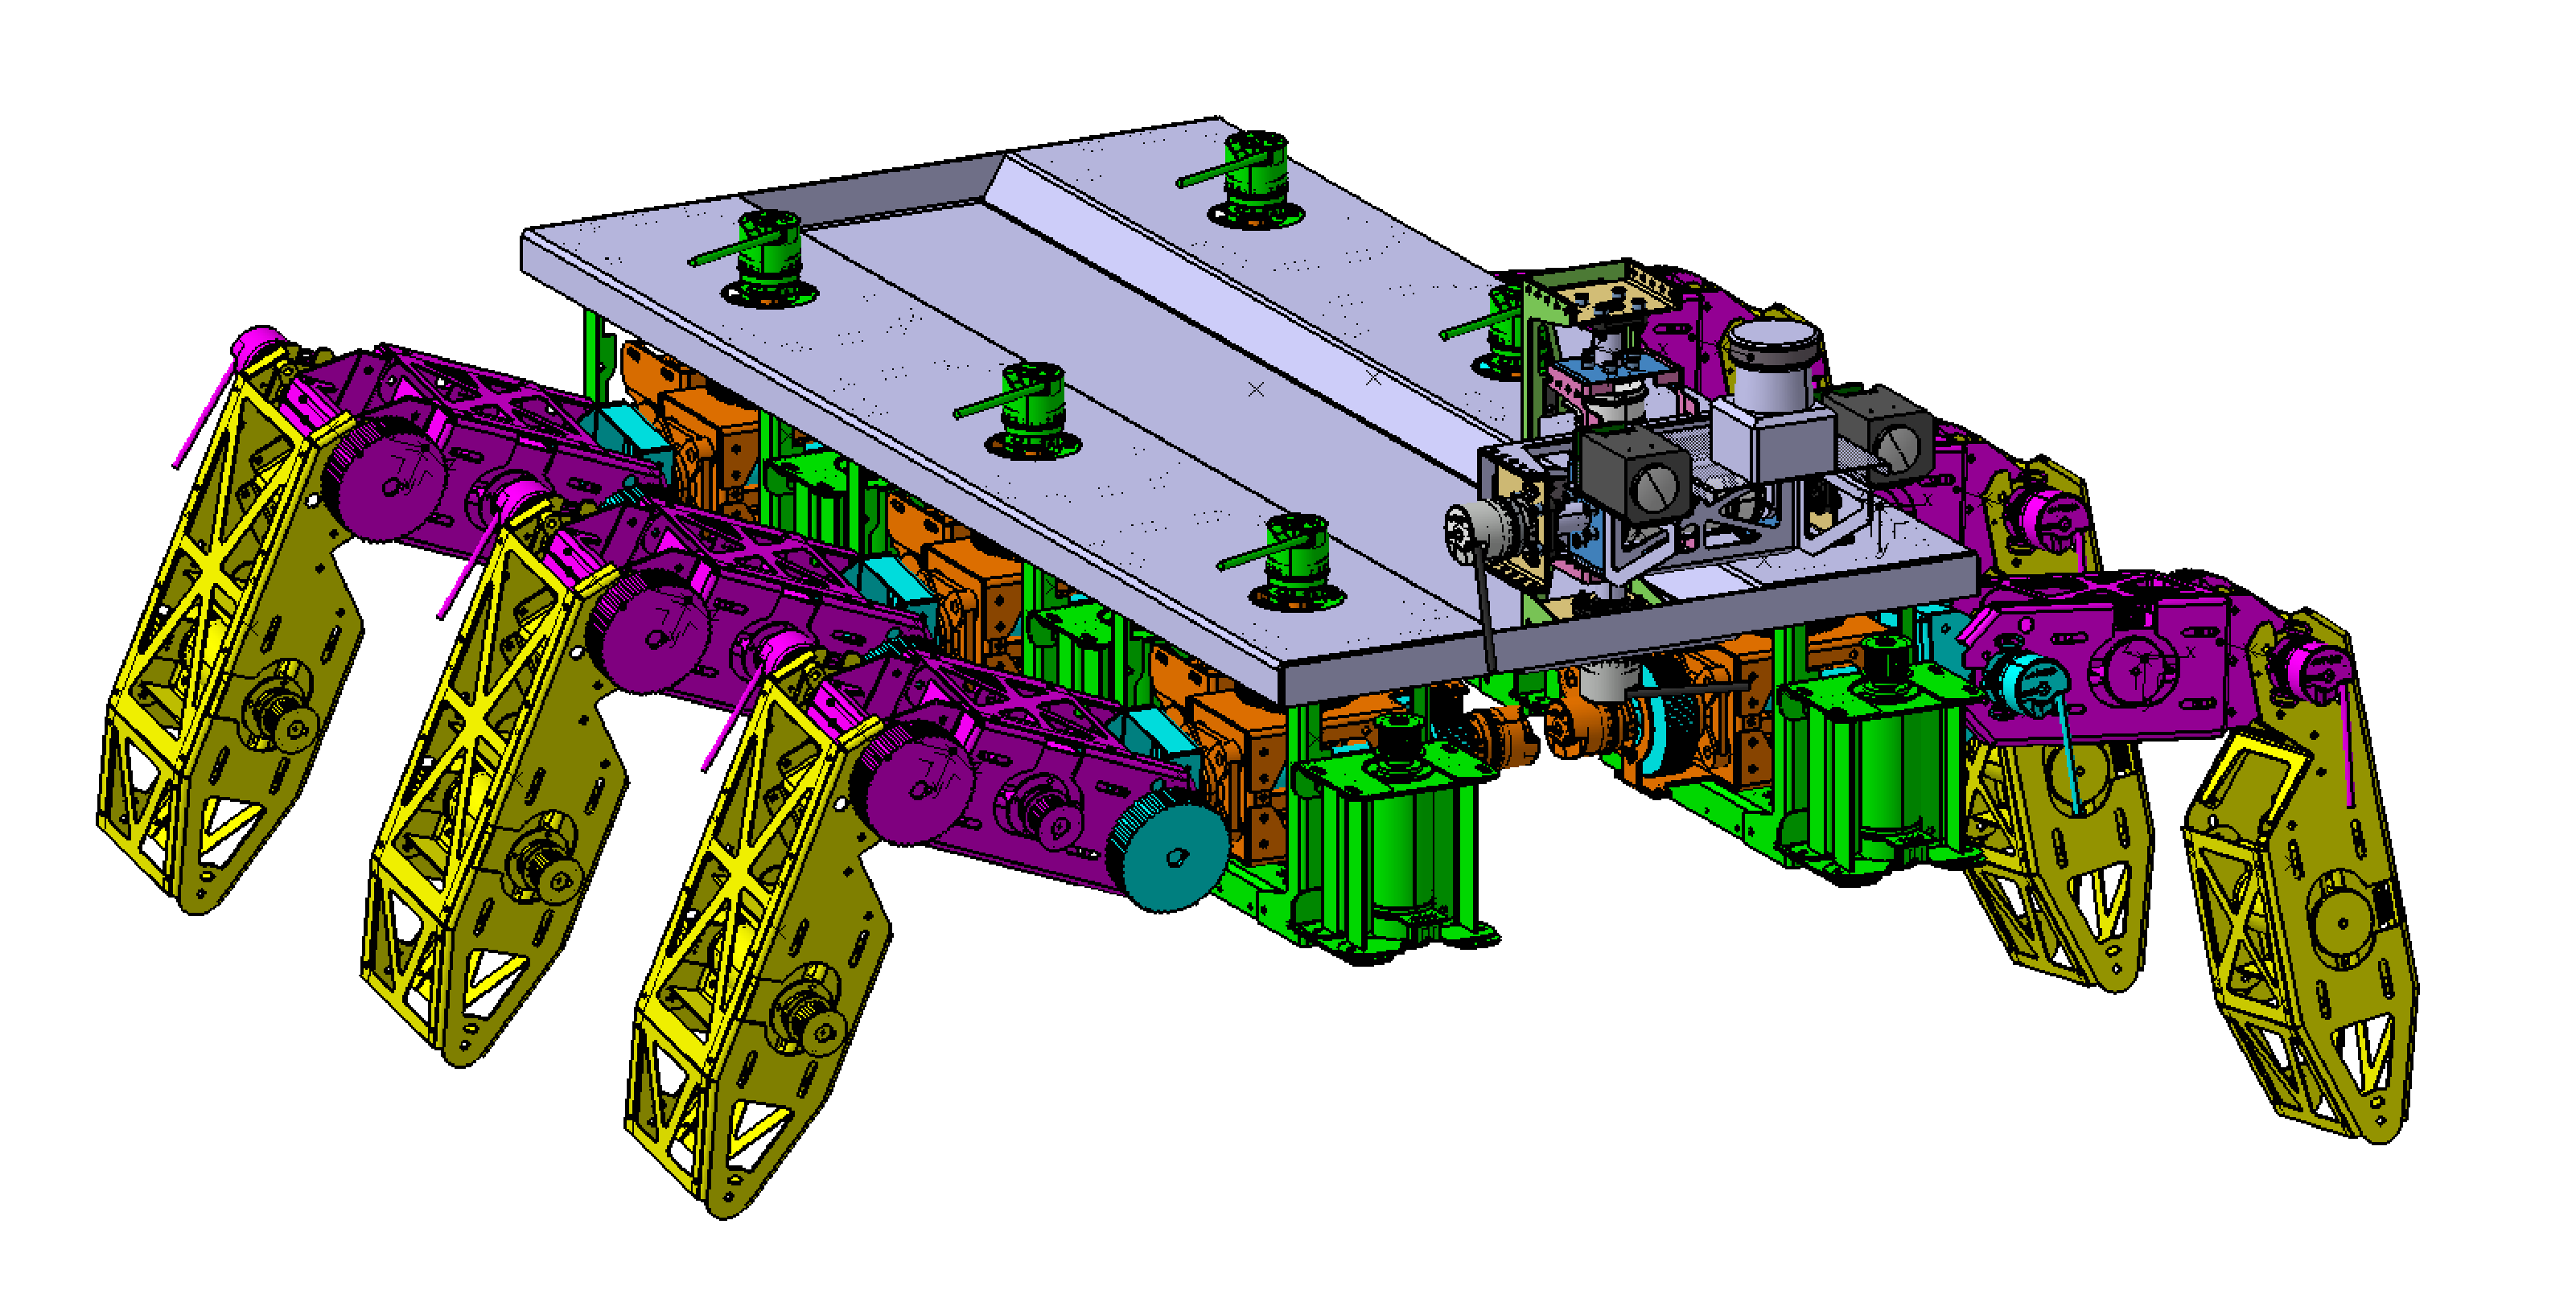
\includegraphics[width = 0.9\columnwidth ]{images/rhex.eps}	
\caption{R.HEX01 CAD Design : General view}
\label{fig_rhex}
\end{figure}

\section{Frame Representation}
\begin{figure}[!htb]
\centering
\includegraphics[width = 0.9\columnwidth ]{images/Rhex_frame_right.eps}	
\caption{Frames for the right foot}
\label{fig_frame_right}
\end{figure}

\newpage
\section{MainBody}

\begin{figure}[!htb]
\centering
\includegraphics[width = 0.9\columnwidth ]{images/MainBody.eps}	
\caption{MainBody CAD Design}
\label{fig_mainbody}
\end{figure}

\begin{table}[h]
\centering
\begin{tabular}{|c||c|}
\hline
Body & MainBody   \\ \hline 
Father & none \\ \hline
Translation from Father frame & \begin{tabular}{ccc} 0.0 & 0.0 & 0.0	\end{tabular} \\ \hline
Rotation from Father frame & \begin{tabular}{ccc} 0.0 & 0.0 & 0.0	\end{tabular} \\ \hline
Mass ($kg$) & 3.174 \\ \hline
Center Of Mass ($m$) & \begin{tabular}{ccc} 0.0 & 0.0 & 0.0	\end{tabular} \\ \hline
Interia ($kg/s^2$) & \begin{tabular}{ccc} 0.291 & 0.0 & 0.0 \\ 0.0 & 0.362 & 0.0 \\ 0.0 & 0.0 & 0.72\end{tabular} \\ \hline
\end{tabular}
\caption{Properties of MainBody}
\end{table}

\newpage
\section{RightShoulder1}

\begin{figure}[!htb]
\centering
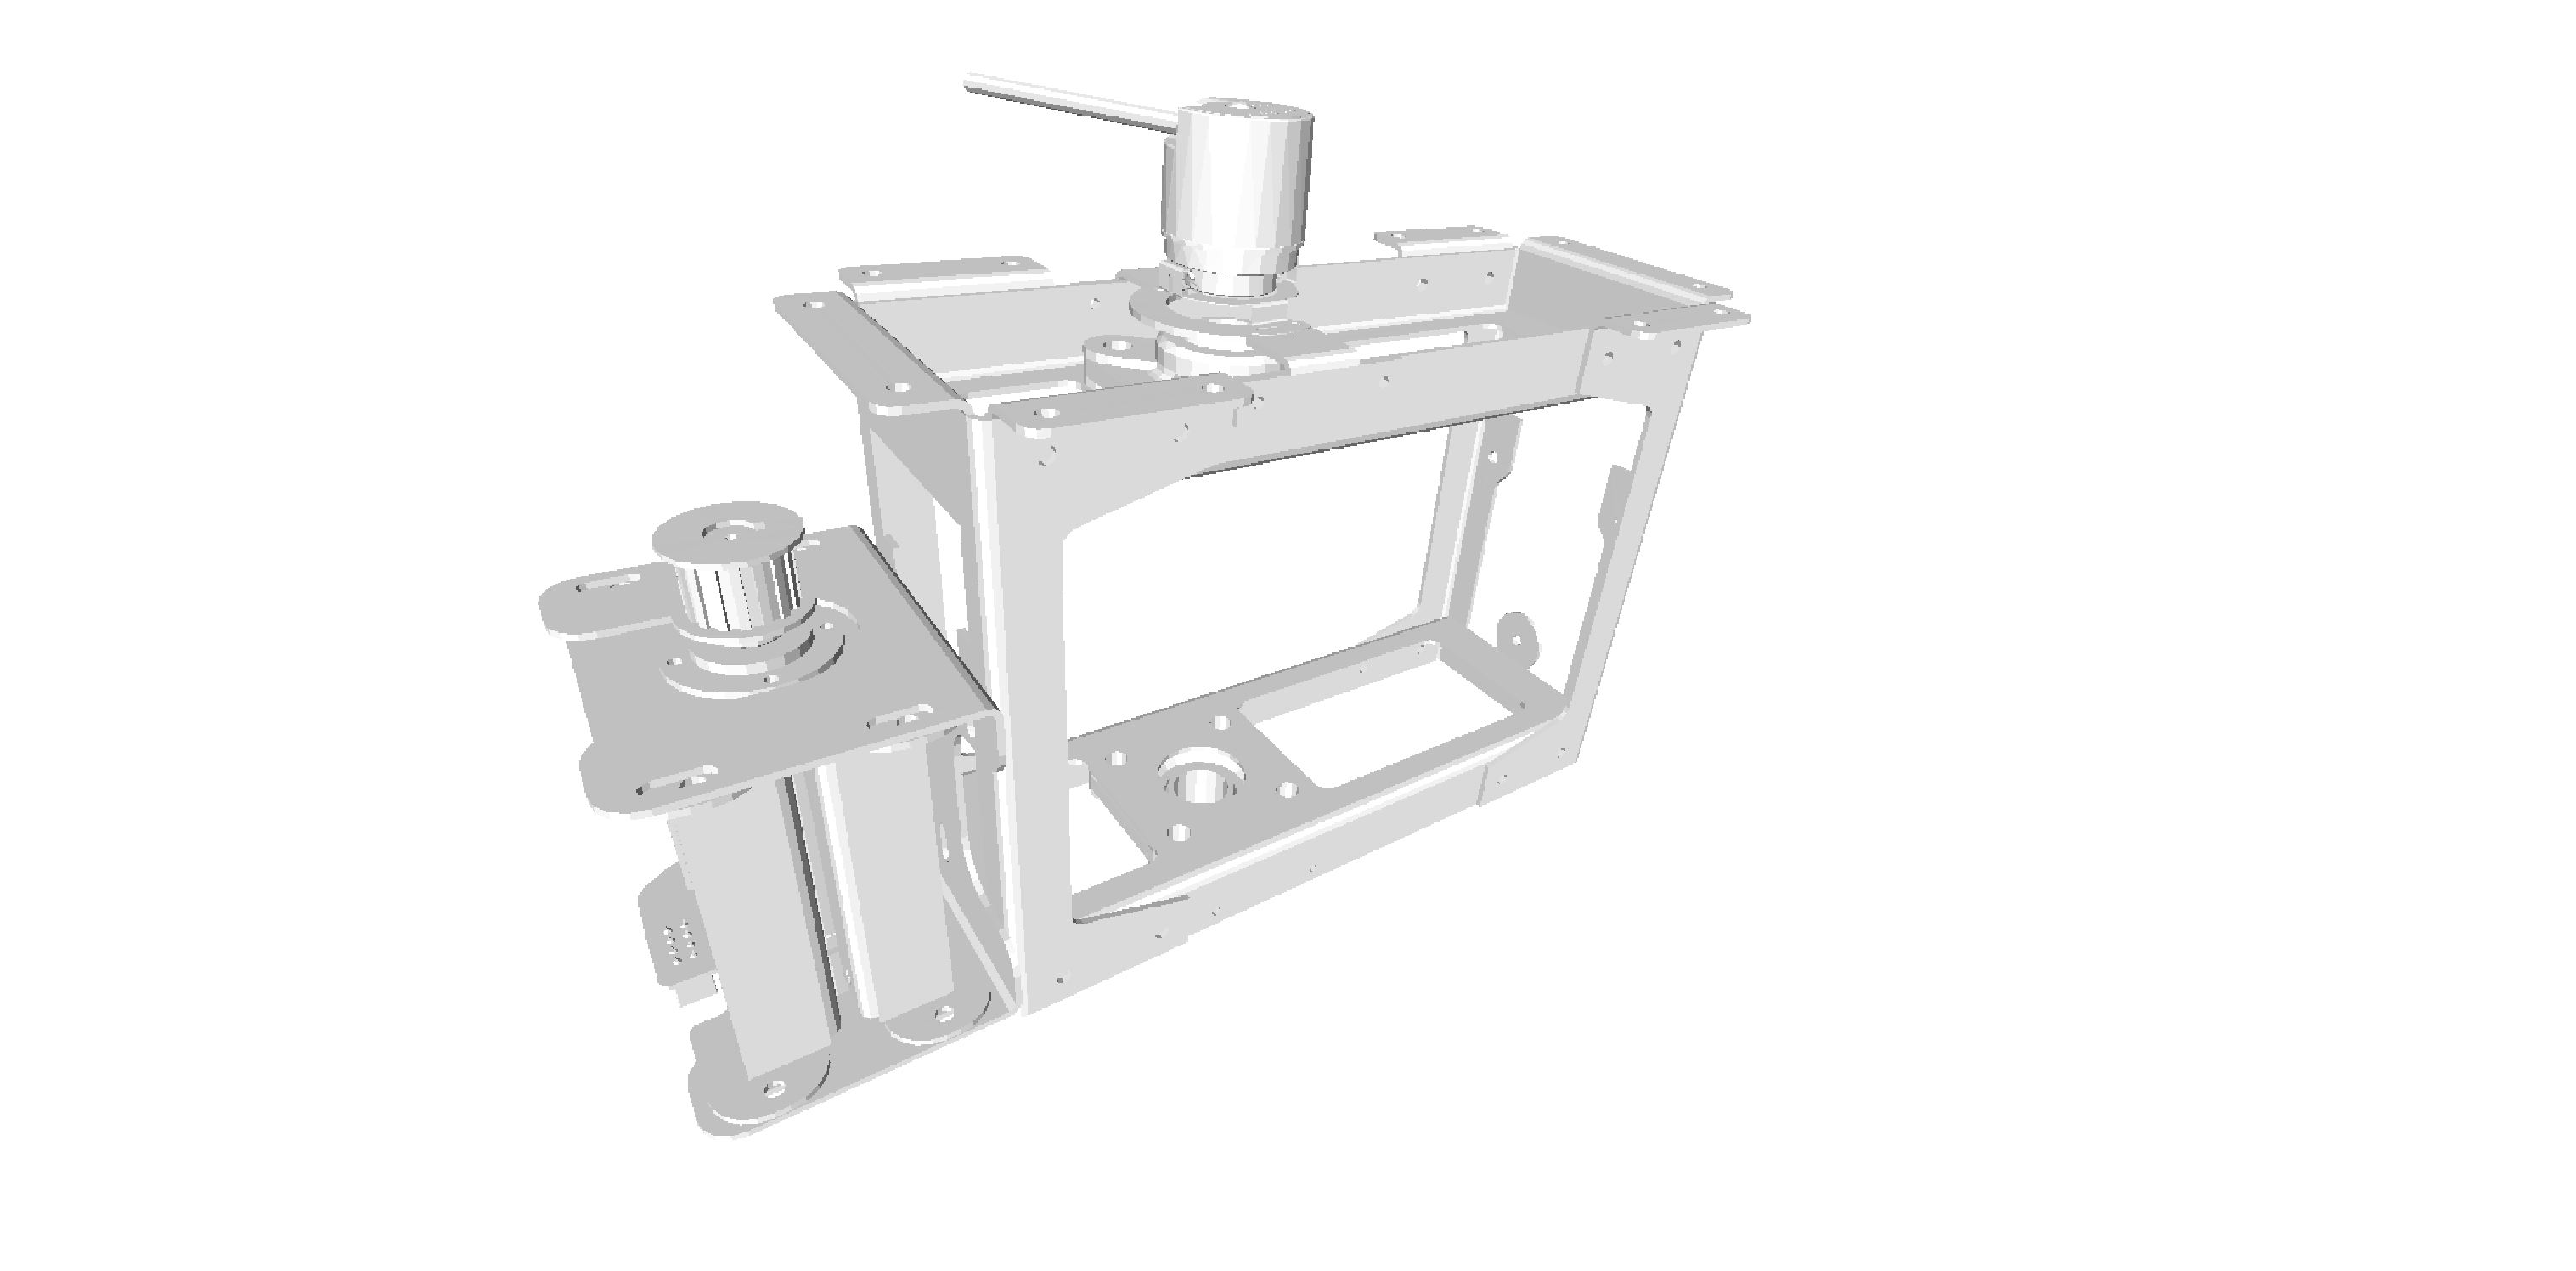
\includegraphics[width = 0.9\columnwidth ]{images/RightShoulder1.eps}	
\caption{RightShoulder1 CAD Design}
\label{fig_RightShoulder1}
\end{figure}

\begin{table}[h]
\centering
\begin{tabular}{|c||c|}
\hline
Body & RightShoulder1   \\ \hline 
Father & MainBody \\ \hline
% Translation from Father frame ($T_x,T_y,T_z$ in meter) & \begin{tabular}{ccc} 0.171 & 0.0 & -0.35 	\end{tabular} \\ \hline
$[T_x,T_y,T_z]$ for front leg & \begin{tabular}{ccc} 0.171 & 0.0 & -0.35 	\end{tabular} \\ \hline
$[T_x,T_y,T_z]$ for middle leg & \begin{tabular}{ccc} 0.0 & 0.0 & -0.35 	\end{tabular} \\ \hline
$[T_x,T_y,T_z]$ for back leg & \begin{tabular}{ccc} -0.171 & 0.0 & -0.35 	\end{tabular} \\ \hline


$[\theta_x,\theta_y,\theta_z]$ & \begin{tabular}{ccc} -90 & 0 & 90 	\end{tabular} \\ \hline
Mass ($kg$) & 2.453 \\ \hline
Center Of Mass ($m$) & \begin{tabular}{ccc} 0.040615 & -0.000338 & 0.013372	\end{tabular} \\ \hline
Interia ($kg/s^2$) & \begin{tabular}{ccc}  0.016 & 0.0 & 0.0004 \\ 0.0 & 0.032 & 0.0001134 \\ 0.004 & 0.0001134 & 0.019  \end{tabular} \\ \hline
\end{tabular}
\caption{Properties of RightShoulder1}
\end{table}

\newpage
\section{RightShoulder2}
\begin{figure}[!htb]
\centering
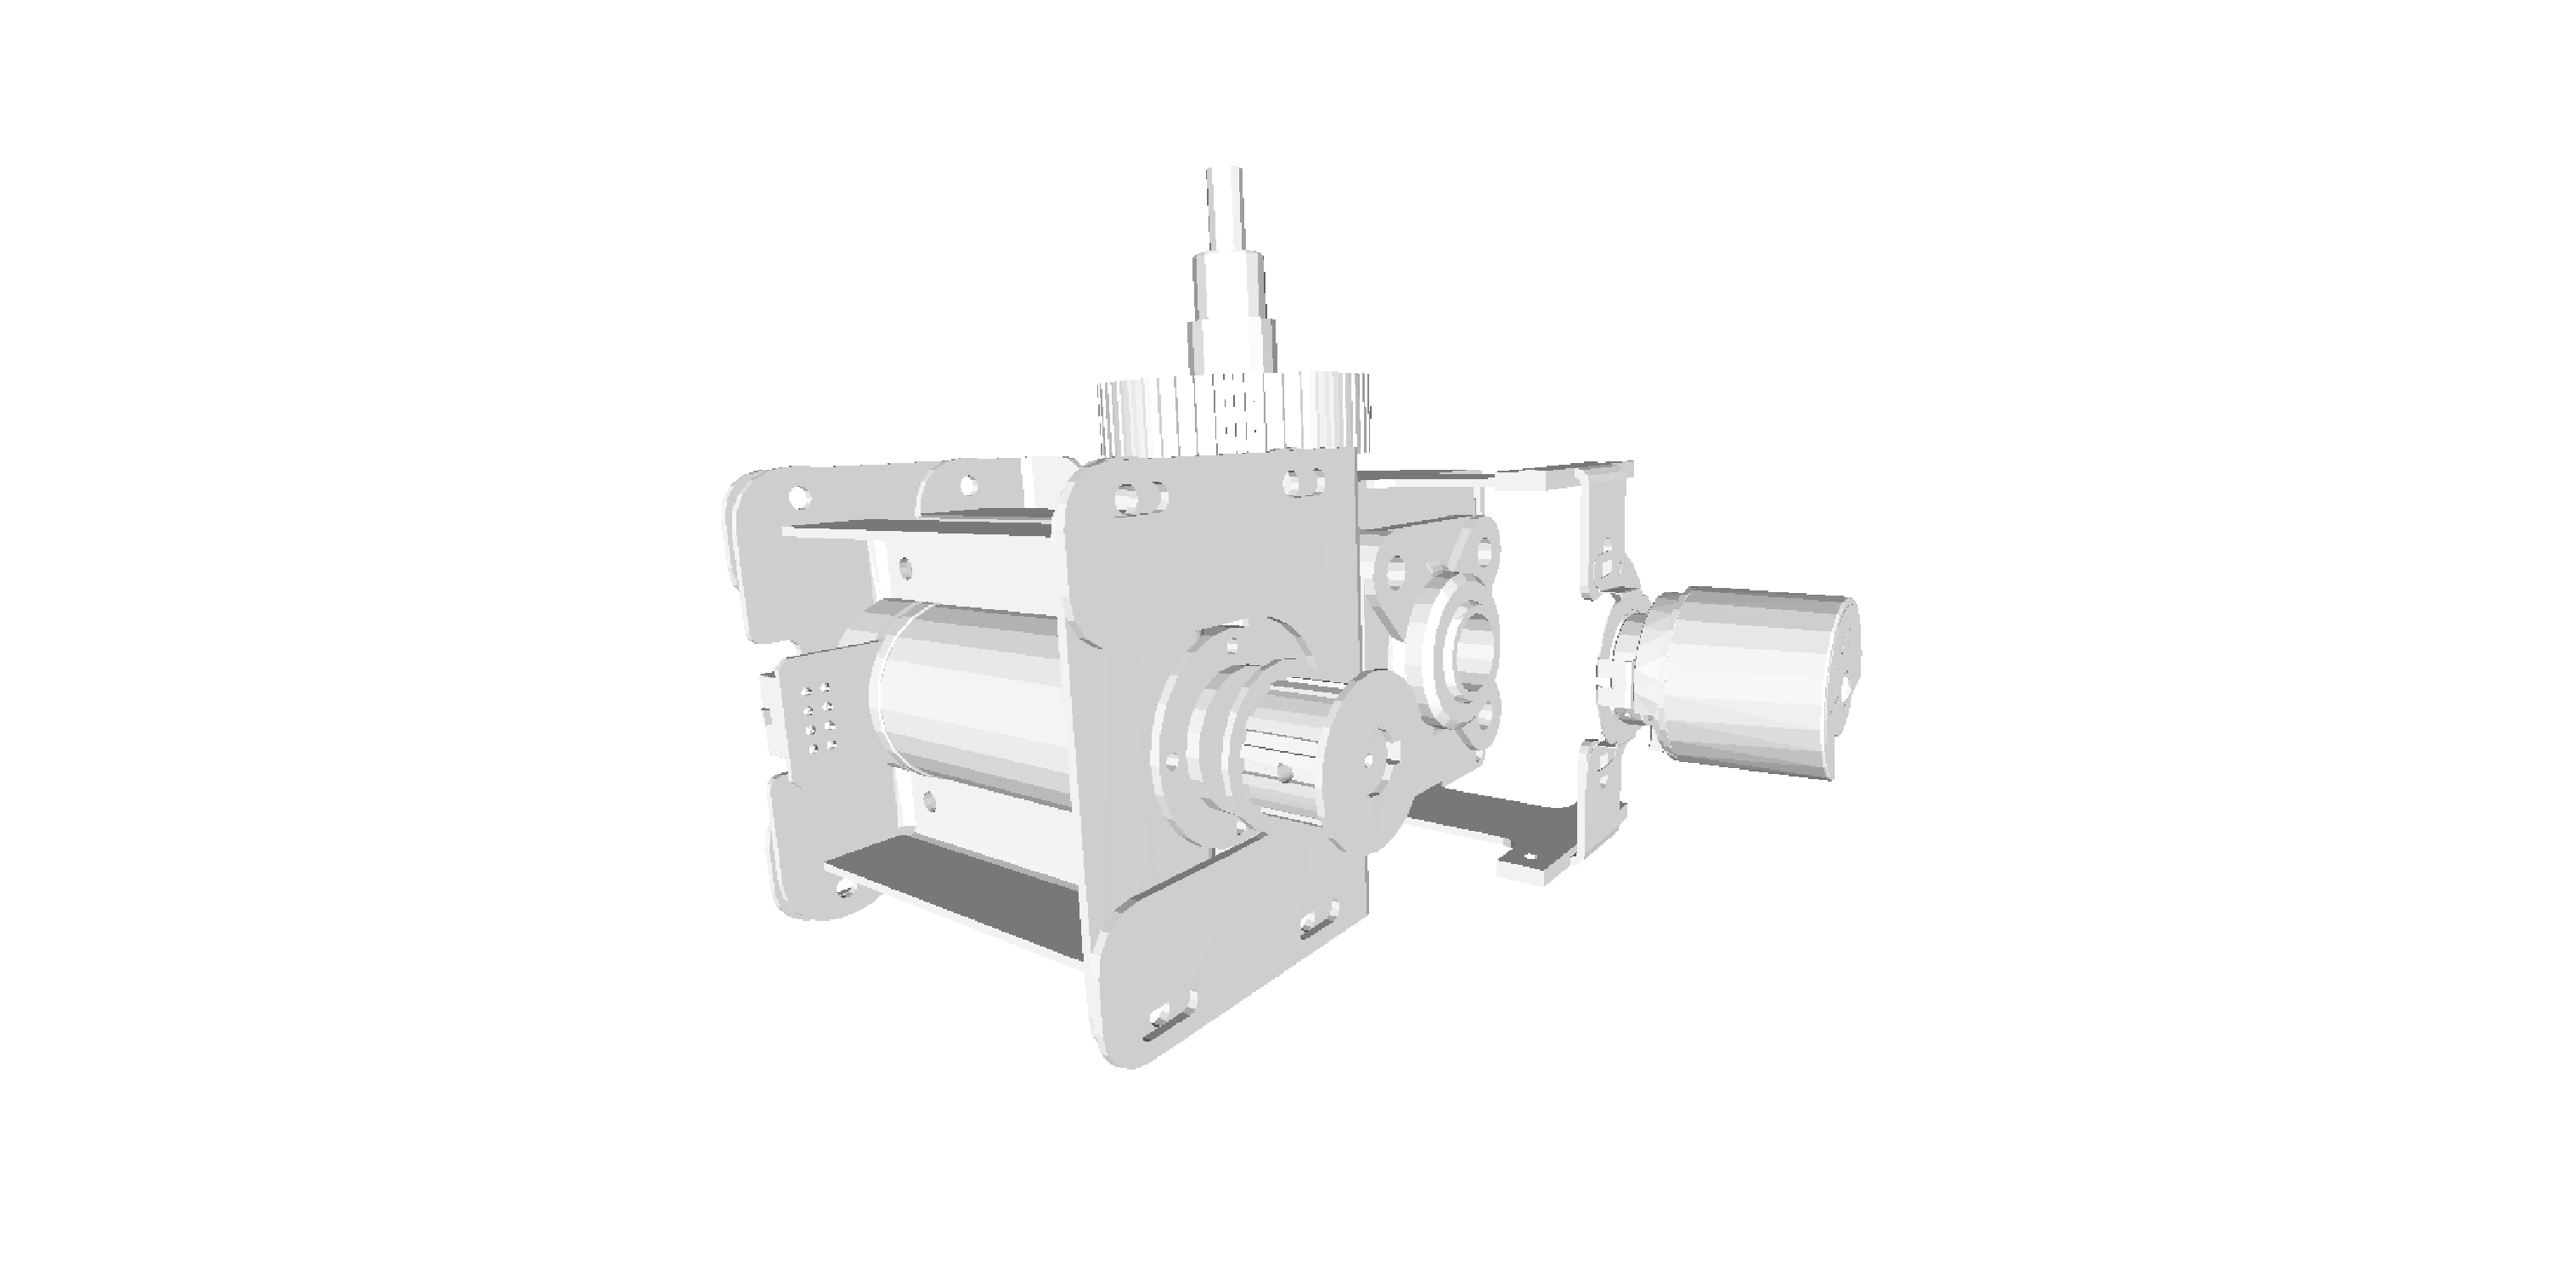
\includegraphics[width = 0.9\columnwidth ]{images/RightShoulder2.eps}	
\caption{RightShoulder2 CAD Design}
\label{fig_RightShoulder2}
\end{figure}

\begin{table}[h]
\centering
\begin{tabular}{|c||c|}
\hline
Body & RightShoulder2   \\ \hline 
Father & RightShoulder1 \\ \hline
$[T_x,T_y,T_z]$ & \begin{tabular}{ccc} 0.0 & 0.0 & 0.0 	\end{tabular} \\ \hline
$[\theta_x,\theta_y,\theta_z]$ & \begin{tabular}{ccc} 0.0 & 0.0 & 0.0 	\end{tabular} \\ \hline
Mass ($kg$) & 2.539 \\ \hline
Center Of Mass ($m$) & \begin{tabular}{ccc} -0.029188 & 0.028369 & -0.005857 	\end{tabular} \\ \hline
Interia ($kg/s^2$) & \begin{tabular}{ccc}  0.012 & 0.0006 & 0.00046 \\ 0.0006 & 0.008 & 0.0005978 \\ 0.0046 & 0.0005978 & 0.015   \end{tabular} \\ \hline
\end{tabular}
\caption{Properties of RightShoulder2}
\end{table}

\newpage
\section{RightShoulder3}
\begin{figure}[!htb]
\centering
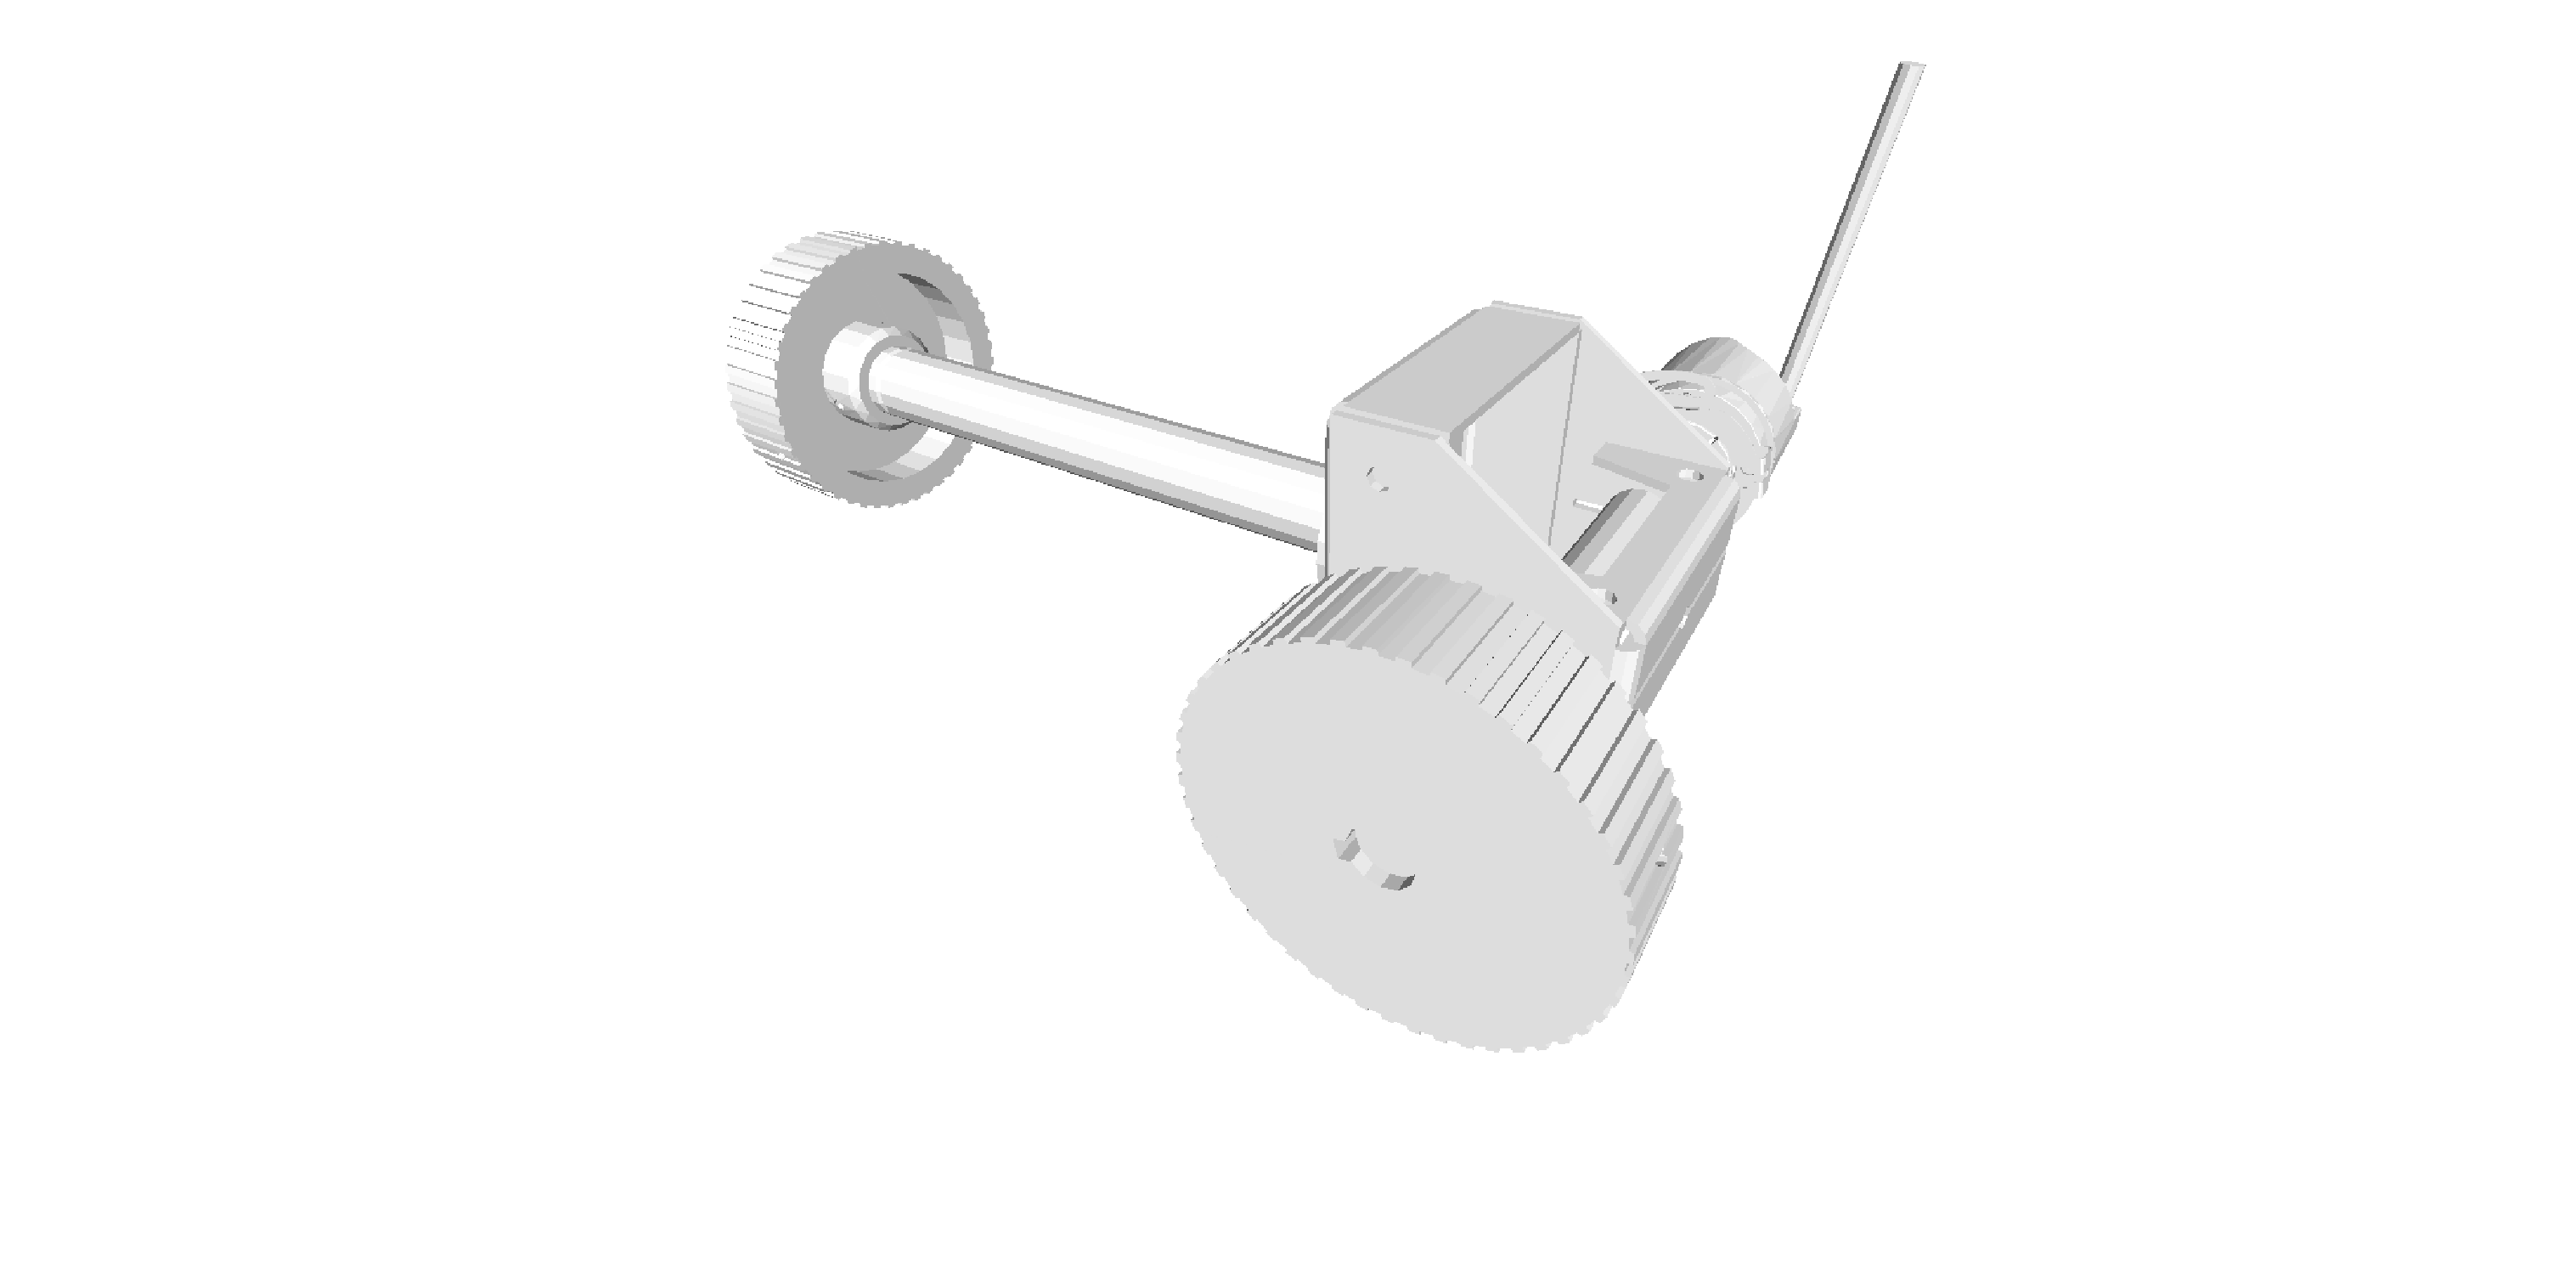
\includegraphics[width = 0.9\columnwidth ]{images/RightShoulder3.eps}	
\caption{RightShoulder3 CAD Design}
\label{fig_RightShoulder3}
\end{figure}

\begin{table}[h]
\centering
\begin{tabular}{|c||c|}
\hline
Body & RightShoulder3   \\ \hline 
Father & RightShoulder2 \\ \hline
$[T_x,T_y,T_z]$ & \begin{tabular}{ccc} 0.0 & 0.0 & 0.127 	\end{tabular} \\ \hline
$[\theta_x,\theta_y,\theta_z]$ & \begin{tabular}{ccc} 0.0 & 90.0 & 0.0 	\end{tabular} \\ \hline
Mass ($kg$) & 1.032 \\ \hline
Center Of Mass ($m$) & \begin{tabular}{ccc} -0.016649 & 0.000981 & -0.073556 \end{tabular} \\ \hline
Interia ($kg/s^2$) & \begin{tabular}{ccc}  0.009 & 0.00009 & -0.00098 \\ 0.000009 & 0.012 & 0.000077 \\ -0.00098 & 0.000077 & 0.004  \end{tabular} \\ \hline
\end{tabular}
\caption{Properties of RightShoulder3}
\end{table}

\newpage
\section{RightArm}
\begin{figure}[!htb]
\centering
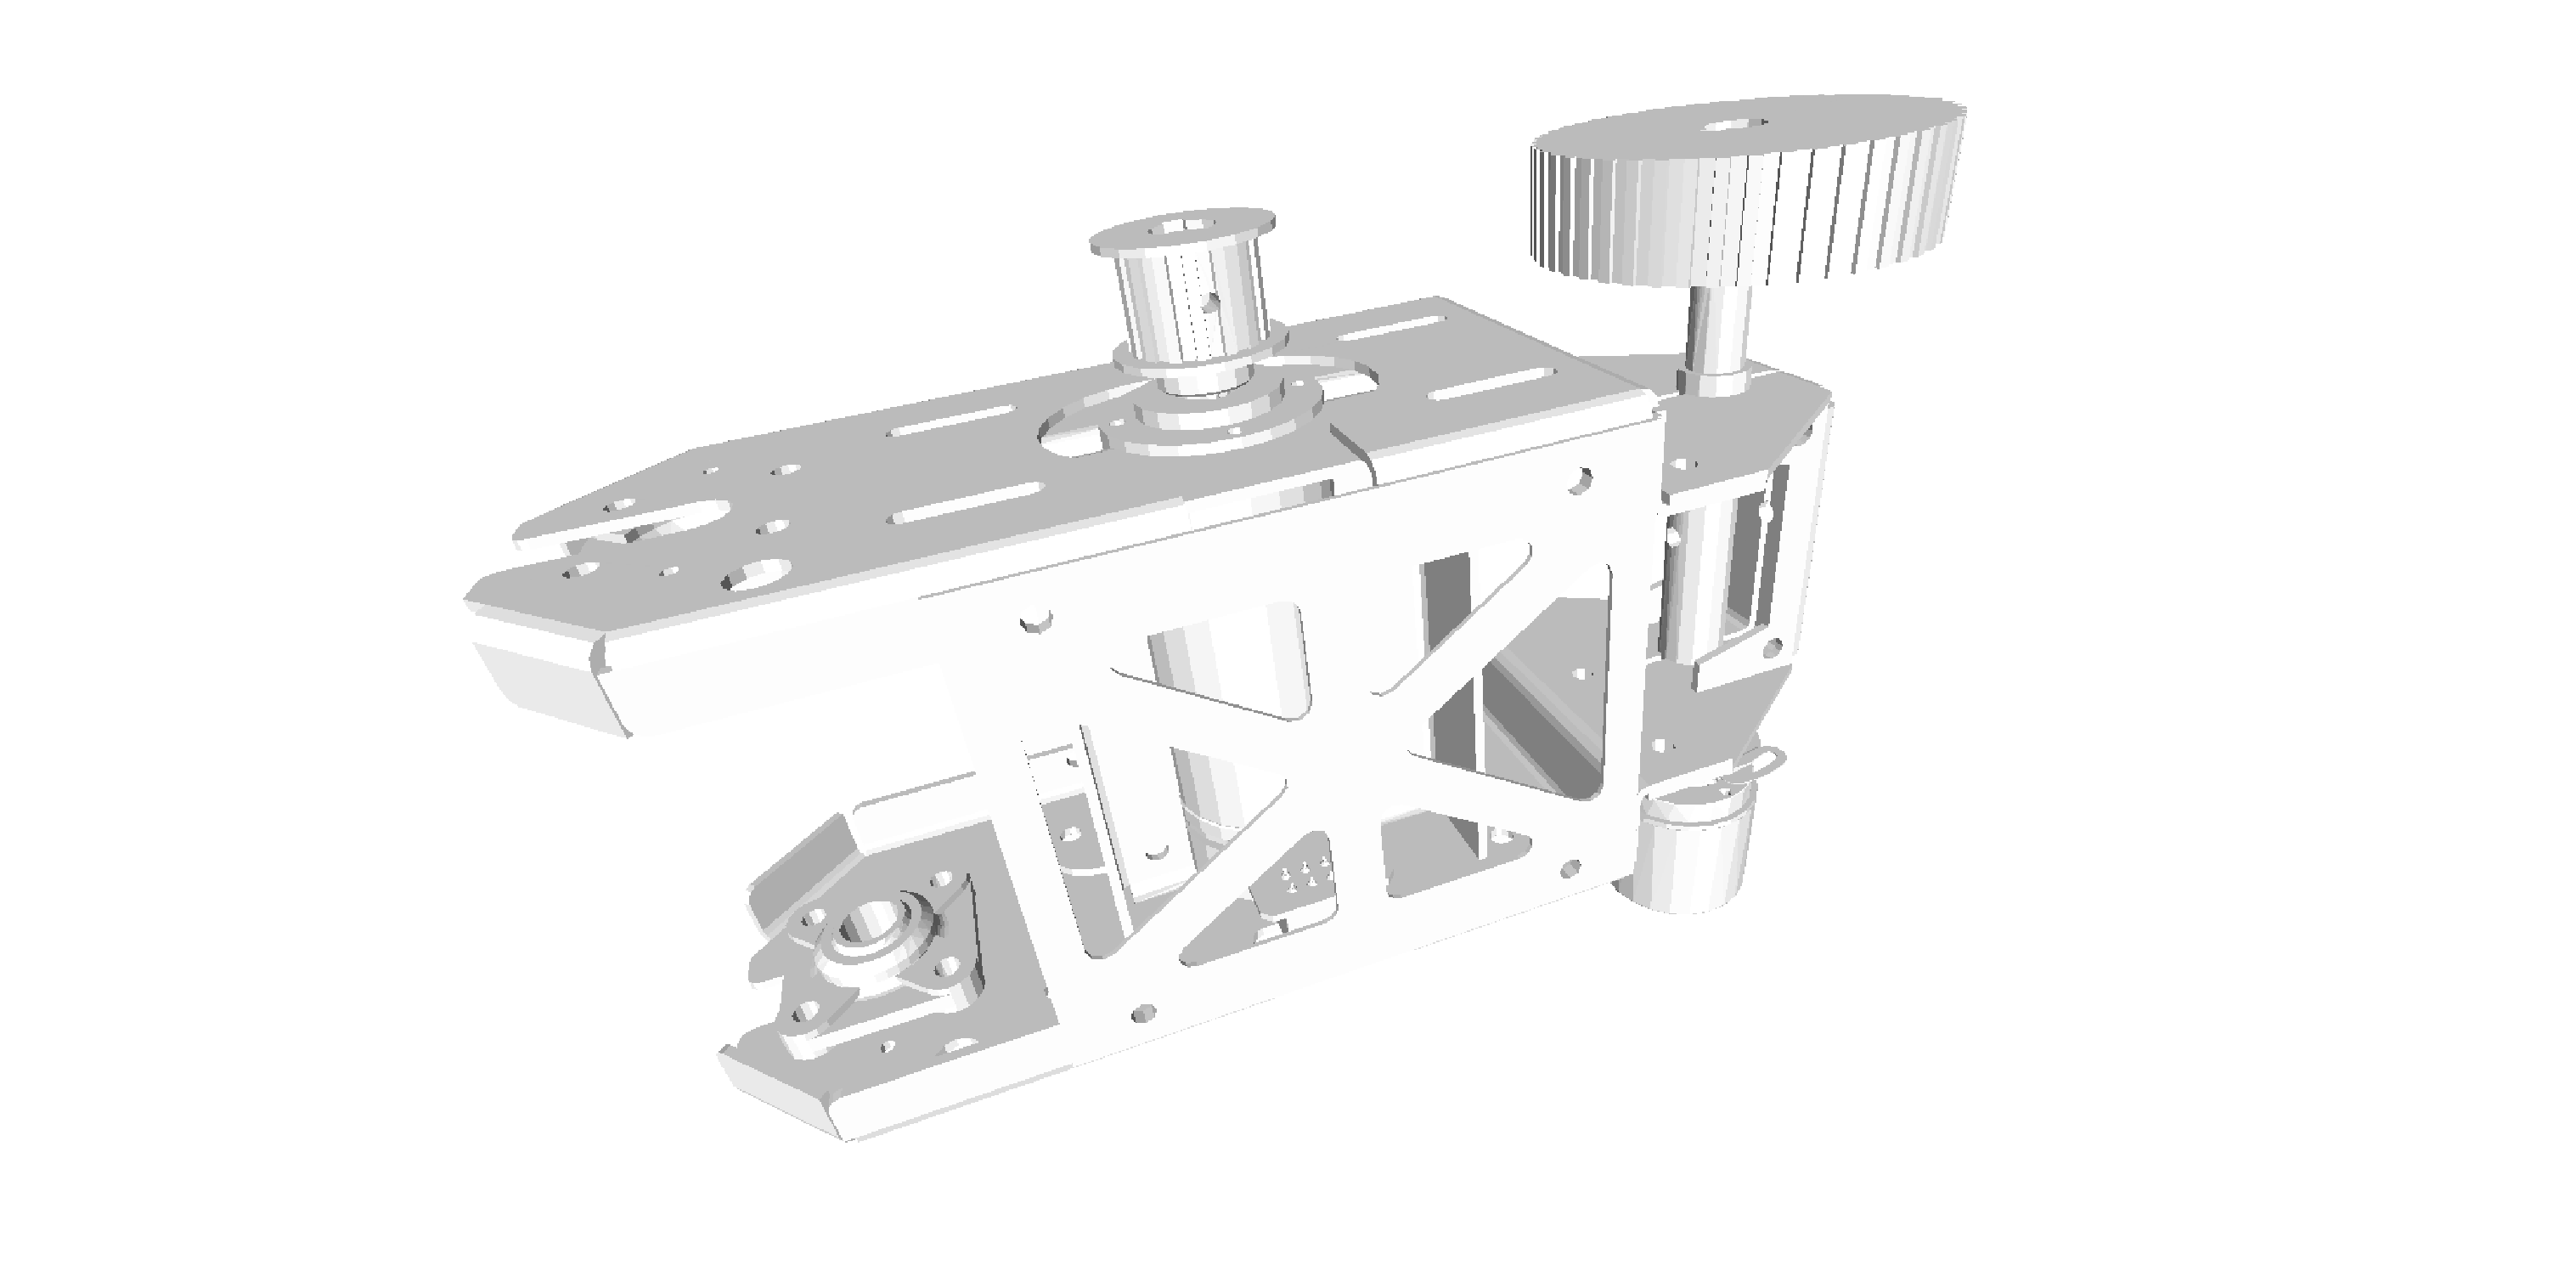
\includegraphics[width = 0.9\columnwidth ]{images/RightArm.eps}	
\caption{RightArm CAD Design}
\label{fig_RightArm}
\end{figure}

\begin{table}[h]
\centering
\begin{tabular}{|c||c|}
\hline
Body & RightArm   \\ \hline 
Father & RightShoulder3 \\ \hline
$[T_x,T_y,T_z]$ & \begin{tabular}{ccc} 0.0 & 0.0 & 0.127 	\end{tabular} \\ \hline
$[\theta_x,\theta_y,\theta_z]$ & \begin{tabular}{ccc} 0.0 & 90.0 & 0.0 	\end{tabular} \\ \hline
Mass ($kg$) & 1.871 \\ \hline
Center Of Mass ($m$) & \begin{tabular}{ccc} 0.121884 & 0.000545 & -0.007791 \end{tabular} \\ \hline
Interia ($kg/s^2$) & \begin{tabular}{ccc}  0.006 & -0.0001 & 0.001 \\ -0.0001 & 0.015 & 0.000088 \\ 0.001 & 0.000088 & 0.01  \end{tabular} \\ \hline
\end{tabular}
\caption{Properties of RightArm}
\end{table}

\newpage
\section{RightForearm}
\begin{figure}[!htb]
\centering
\includegraphics[width = 0.9\columnwidth ]{images/RightForearm.eps}	
\caption{RightForearm CAD Design}
\label{fig_RightForearm}
\end{figure}

\begin{table}[h]
\centering
\begin{tabular}{|c||c|}
\hline
Body & RightForearm   \\ \hline 
Father & RightArm \\ \hline
$[T_x,T_y,T_z]$ & \begin{tabular}{ccc} -0.2 & 0.0 & 0.0 	\end{tabular} \\ \hline
$[\theta_x,\theta_y,\theta_z]$ & \begin{tabular}{ccc} 0.0 & 0.0 & 90.0 	\end{tabular} \\ \hline
Mass ($kg$) & 1.287 \\ \hline
Center Of Mass ($m$) & \begin{tabular}{ccc} 0.140274 & 0.001512 & -0.002044 \end{tabular} \\ \hline
Interia ($kg/s^2$) & \begin{tabular}{ccc}  0.003 & 0.0001876 & 0.00007837 \\ 0.0001876 & 0.009 & -0.00001543 \\ 0.00007837 & -0.00001543 & 0.008  \end{tabular} \\ \hline
\end{tabular}
\caption{Properties of RightArm}
\end{table}


\newpage
\chapter{Test procedure of the design}
\minitoc
 


\end{document}          
